%% bare_jrnl.tex
%% V1.3
%% 2007/01/11
%% by Michael Shell
%% see http://www.michaelshell.org/
%% for current contact information.
%%
%% This is a skeleton file demonstrating the use of IEEEtran.cls
%% (requires IEEEtran.cls version 1.7 or later) with an IEEE journal paper.
%%
%% Support sites:
%% http://www.michaelshell.org/tex/ieeetran/
%% http://www.ctan.org/tex-archive/macros/latex/contrib/IEEEtran/
%% and
%% http://www.ieee.org/

\documentclass[journal,a4paper,oneside,twocolumn]{IEEEtran}

\usepackage[portuguese]{babel}
\usepackage[utf8]{inputenc}

\usepackage{natbib}

\ifCLASSINFOpdf
  \usepackage[pdftex]{graphicx}
  % declare the path(s) where your graphic files are
 % \graphicspath{{../Figs/}
  % and their extensions so you won't have to specify these with
  % every instance of \includegraphics
  \DeclareGraphicsExtensions{.pdf,.jpeg,.png}
\else
  % or other class option (dvipsone, dvipdf, if not using dvips). graphicx
  % will default to the driver specified in the system graphics.cfg if no
  % driver is specified.
  % \usepackage[dvips]{graphicx}
  % declare the path(s) where your graphic files are
  % \graphicspath{{../eps/}}
  % and their extensions so you won't have to specify these with
  % every instance of \includegraphics
  % \DeclareGraphicsExtensions{.eps}
\fi

\usepackage{multirow}
\usepackage[disable]{todonotes}


%\usepackage[colorinlistoftodos]{}  
\setlength{\marginparwidth}{1cm}
%\reversemarginpar

% correct bad hyphenation here
\hyphenation{op-tical net-works semi-conduc-tor}

%\renewcommand{\IEEEkeywords}{\textbf{Palavras chave -} 

\begin{document}
%
% paper title
% can use linebreaks \\ within to get better formatting as desired
\title{ Sistema De Controle Em Tempo Real Reconfigur\'{a}vel De 
		Experimento Em Astrobiologia }

\author{
		Rafael~Corsi~Ferr\~{a}o, 
        Tiago~Sanches~Da~Silva,
        Sergio~Ribeiro~Augusto,
        Vanderlei~Cunha~Parro$^{a}$ 
        \\%   <-this % stops a space
        Instituto Mau\'{a} de Tecnologia -  N\'{u}cleo de Sistemas Eletr\^{o}nicos Embarcados \\
        S\~{a}o Caetano do Sul - SP - Brazil 
        
\thanks{ $^{a}$Autor para correspondência: Vanderlei~Cunha~Parro, E-mail: vparro@mac.com .}% <-this % stops a space
}
%\thanks{Manuscript received April 19, 2005; revised January 11, 2007.}}


% The paper headers
%\markboth{Journal of \LaTeX\ Class Files,~Vol.~6, No.~1, January~2007}%
%{Shell \MakeLowercase{\textit{et al.}}: Bare Demo of IEEEtran.cls for Journals}


\maketitle


\begin{abstract}
	Este trabalho apresenta uma arquitetura de um sistema em tempo real e reconfigurável para controle de experimentos em aplicações aeroespacial. A arquitetura de software proposta tem como base dois tipos de serviços: o PBS (\textit{Primary Boot Service}), o qual é responsável pela inicialização do sistema bem como sua reconfiguração e atualização remota, e o APS (\textit{Application Service}), responsável por controlar as diversas partes dos  experimentos e também pela comunicação com a plataforma. Ao  final do artigo é apresentando uma topologia baseada no processador Leon e no protocolo espacial SpaceWire desenvolvida para a implementação da arquitetura proposta.
	
%	visa a concepção e implementação de um sistema operacional com
%	características de tempo real e reconfigurável, para aplicações em experimentos espaciais,
%	sendo parte do projeto de pesquisa “Sistema de Controle de Tempo Real Reconfiguravel em
%	Astrobiologia”, financiado pela Agência Espacial Brasileira (AEB). O sistema operacional
%	será implementado em processador LEON [1] com arquitetura ternária adequada a
%	aplicações que envolvem alta confiabilidade. A arquitetura de software proposta tem como
%	base dois tipos de serviços: o PBS (Primary Boot Service), o qual é responsável pela
%	inicialização do sistema bem como sua reconfiguração e atualização remota, e o APS
%	(Aplication Service), responsável por controlar experimentos, sensores e atuadores. Este
%	último tem como objetivo preparar os dados para enviar a uma base terrestre.		
\end{abstract}

% Note that keywords are not normally used for peerreview papers.
\begin{IEEEkeywords}
	RTOS, Leon, Sistema Reconfigurável, SpaceWire, 
\end{IEEEkeywords}


\IEEEpeerreviewmaketitle



\section{Introdução}

	\IEEEPARstart{C}{om} o aumento da complexidade de experimentos embarcados em aplicações aerospaciais surge a demanda do desenvolvimento de uma arquitetura de software capaz de suprir as necessidades de um experimento científico  de tempo real, e que possa ser remotamente atualizado em partes ou total.
	%reconfigurado  para uma nova versão, 
	Essa necessidade é baseada no fato de que correções ou melhorias no software pós lançamento pode corrigir falhas que o experimento possa sofrer durante seu tempo de operação podendo assim aumentando  a vida útil do experimento e/ou a qualidade dos resultados.
	
	 A presente plataforma foi inspirada do ponto de vista de protocolos e sub sistemas no satélite CoRoT\footnote{\textit{COnvection ROtation et Transits planétaires}} \cite{cailliau1999corot}, com enfoque no experimento de Astrobiologia proposto para ser  embarcado na primeira sonda de espaço profundo brasileira (Aster). 
	 
	 Esta proposta implica em definir claramente  as interfaces de comunicação e o sistema operacional da carga útil. Sistemas para aplicações aerospaciais são geralmente implementado com funcionalidade bem definida visando aumentar a robustez da aplicação. 	Entende-se por aumento de robustez a capacidade do software  de não causar situações que possam interromper, parcialmente ou totalmente, o funcionamento do experimento quando em modo de operação. 
	 
	 O sistema proposto é baseado em quatro serviços:  o PBS (\textit{Primary Boot Service}), responsável pelo sistema de boot após reinicio físico, permite uma manipulação mínima do sistema de processamento e inclui o kernel das funções elementares	 do software bem como a verificação da integridade do código no APS e suas atualizações. E o APS (\textit{Application Service}) serviço relativo a aplicação,ou seja, o gerenciamento do experimento propriamente dito. O mesmo possibilita telemetria. Este serviço pode ser atualizado e reconfigurado, essa tarefa é executada pelo PBS. O Monitor de comunicação externa é responsável pelo gerenciamento da comunicação e o Sistema de controle de experimentos que gerência em baixo nível os experimentos.
	 
	 Foi escolhido como meio de comunicação entre experimento e plataforma o protocolo SpaceWire (SpW) \cite{SpW}, amplamente utilizado em missões espaciais possui grande aderência internacional pelo fato de possuir alta taxa de transmissão atrelado a um baixo consumo energético. 
	 
	O processador Leon 3 \cite{LEON3} foi escolhido como plataforma de desenvolvimento do software proposto. É um processador amplamente utilizado em missões espaciais \cite{abbasitabar2012susceptibility}, vem sendo estudado pelo INPE como  sucessor dos processadores atualmente em uso.
	
\section{Arquitetura do Software}
		
	A proposta visa a criação de uma arquitetura capaz de ser utilizada em diferentes tipos de experimento.   	
	O software foi estruturado com base em dois serviços básicos (Fig \ref{fig:arq}), onde cada serviço possui três estados de operação, sendo apenas um estado de cada serviço é executado simultaneamente. O sistema utiliza como base de implementação um sistema operacional de tempo real (RTOS) como o RTEMS \cite{zhang2010research}, utilizando suas funcionalidades de multi-tarefas, comunicação entre-tarefas e escalonamento entre tarefas.
	
	Definiu-se quatro 
	
	\begin{figure}[!t]
	\centering
	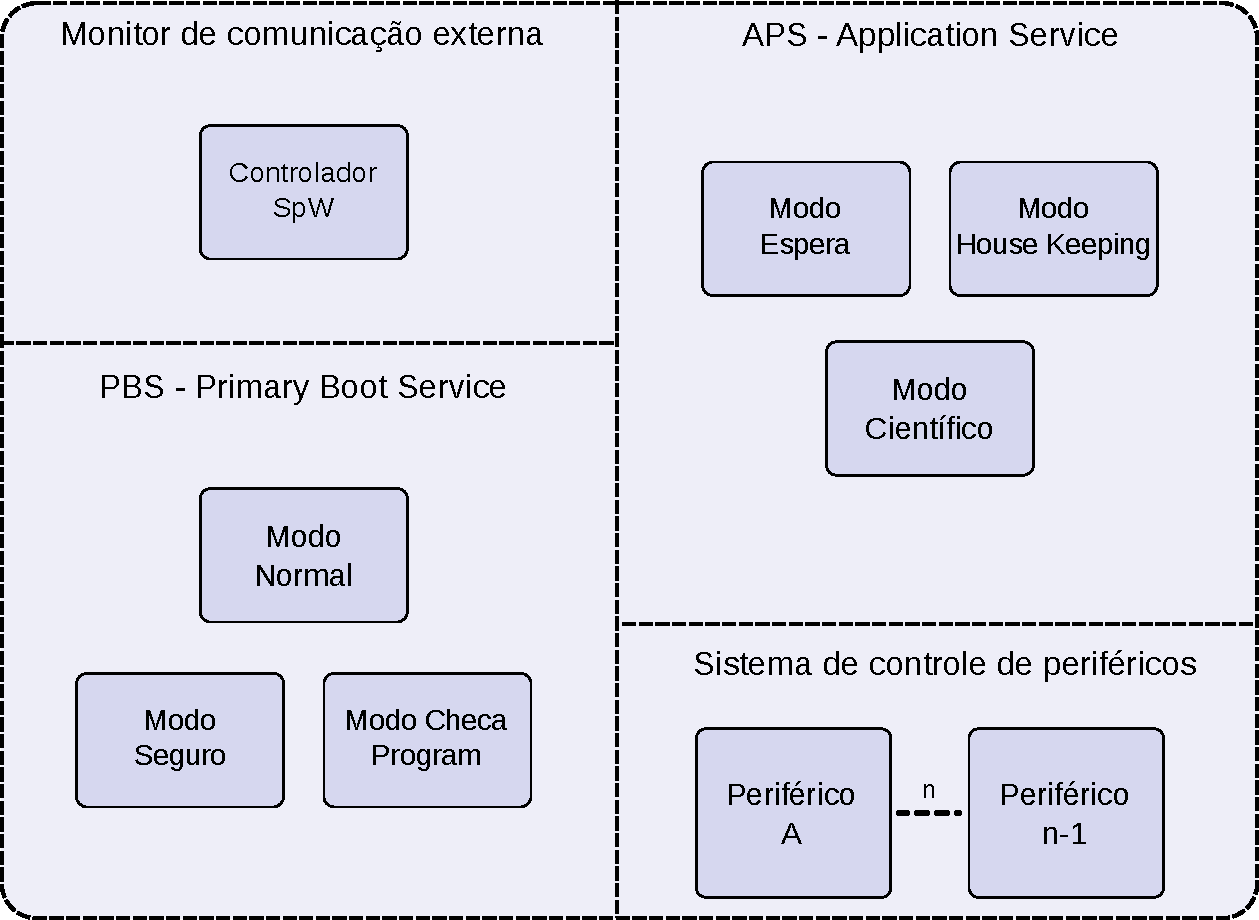
\includegraphics[width=1 \columnwidth,]{Figs/arquitetura.pdf}
	\caption{Diagrama de Harel do sistema  proposto}
	\label{fig:arq}
	\end{figure}
	
\subsection{Monitor de comunicação externa}
	
	O monitor de comunicação externa é uma tarefa responsável pelo controle, codificação/decodificação dos telecomandos (TC) que são enviados e recebidos pelo experimento. Como forma de comunicação, foi escolhido o protocolo SpaceWire, porém outras alternativas tais como o protocolo MIL-1553 \cite{mil1553} podem ser emprega.
	
	As alterações de estados ocorrem por telecomando enviados da plataforma ao experimento,  os TC são interpretados pelo módulo de comunicação que implementa um protocolo baseado em comando/resposta (ack) . Os comandos interpretados pelo módulo de comunicação são colocados em uma fila no experimento \todo{não há prioridade nos comandos ?}. Após a	realização da operação, sendo bem sucedida ou não, o experimento envia uma resposta a	respeito da operação, o que chamamos neste trabalho de OReply (Operational Reply). O diagrama do modelo do OReply é mais simples que o de envio de comando, pois não existe a	necessidade de reenvios e respostas, o OReply é encarado apenas como informativo, ou seja,	não é um tipo de comunicação critica.
	
	O datagrama desenvolvido para comunicação é subdividido em três partes, cabeçalho, comando e parâmetros, totalizando 8 bytes, como demonstrado na Tab. \ref{tab:datagrama}. O Cabeçalho, composto por três partes: possui o \textit{Identificador} do comando que é um valor único que identifica o datagrama; \textit{Tipo} o qual define se o datagrama é do tipo ack ou OReply; \textit{Tamanho} indicando a quantidade de dados que a mensagem possui. A parte do datagrama que diz respeito ao \textit{Comando} identifica o comando a ser executado pelo sistema. Nos parâmetros: \textit{Serviço} indica para qual tarefa o comando está sendo direcionado e os \textit{Parâmetros} são utilizado para complementar alguns comandos, como por exemplo, o comando inicializar, que que envia como parâmetro a versão do firmware a ser inicializado.
	
	
	
\begin{table}[!t]
\centering
		\begin{tabular}{ c c c}
			 & Conteúdo  \\
			\hline 
			
			\multirow{3}{*}{Cabeçalho} 
			& Identificador \\  
			& Tipo \\  
			& Tamanho \\
			
			\multirow{1}{*}{Comando} 
			& Id \\  
			
			\multirow{4}{*}{Parâmetro} 
			& Serviço \\  
			& Parâmetro 1 \\  
			& Parâmetro 2 \\  
			& Parâmetro 3 \\  
			
			\end{tabular} 
			\caption{Estrutura do datagrama proposto}
			\label{tab:datagrama}
\end{table}

\subsection{PBS}	

	 O PBS é o controlador geral do experimento, nele estão o núcleo do sistema operacional e todas as tarefas críticas, não sendo reconfigurável. Os possíveis estados de operação são :
		
		\begin{itemize}
			\item \textbf{Modo Normal }- Executa uma versão do APS na inicialização do sistema e recebe 	comandos externos da comunicação, sendo que estes comandos servem para mudar o PBS ou	o APS de estado;
						
			\item \textbf{Modo Seguro} - O PBS entra neste modo para atualizar o código do APS ou parte dele. Este modo não pode ser acionado no meio de uma operação de risco do APS, ou seja, quando APS estiver interagindo diretamente com os sensores e atuadores;
			
			\item \textbf{Modo Checa Programa} - Modo onde é verificado se o código gravado na EEPROM (APS) está íntegro e sem alterações.
		\end{itemize}

	Na inicialização do sistema, o PBS é colocado em Modo Checa Programa, onde verifica se a última versão do software armazenada na memória está integro. Verificada essa informação passa-se para o Modo Normal, onde inicializa-se o APS , possibilitando que comandos sejam transmitidos para o APS e que atualizações possam ser enviadas ao PBS.

\subsection{APS}		

	O APS é o serviço relativo ao gerenciamento do experimento propriamente dito. O mesmo possibilita telemetria de aquisição de dados dos sensores e varredura do instrumento para verificação de sua integridade. Este serviço pode ser atualizado e reconfigurado pela plataforma, possui os seguintes modos de operação:

	\begin{itemize}
		\item \textbf{Modo de Espera} - Este modo monitora a comunicação entre tarefas de maneira a verificar a existência de comandos enviados da plataforma para o APS;
		
		\item \textbf{Modo Housekeeping} - Este modo é responsável pela varredura dos sensores e atuadores do experimento, verificando se estão comunicáveis e íntegros;
		
		\item \textbf{Modo Científico} - Responsável pela operação do experimento. Também realiza o empacotamento das informações geradas pela telemetria para que seja enviada para a plataforma ou armazenada em memória.
	\end{itemize}
	
\subsection{Sistema de controle de periféricos}

	O sistema de controle de periféricos é um conjunto de tarefas, responsáveis pelo controle dos diversos periféricos do experimento. Esses periféricos podem ser atuadores, sensores ou memórias. Cada periférico é controlado por uma ou mais tarefas, flexibilizando a arquitetura. Os modos de operação de cada periférico são controlados individualmente pelo modo de operação do APS.
	
\subsection{Alocação de memória}

	A alocação de memória proposta para o sistema, possui arquitetura ilustrada na Fig. \ref{fig:mem}, onde são utilizados uma memória somente de leitura (MRAM), e outra volátil (SRAM). Os serviços críticos do sistema, formados pelo PBS e pelo Monitor de comunicação externa são armazenados. Já as partes reconfiguráveis e as varáveis de programa são armazenadas na memória SRAM.

	\begin{figure}[!t]
	\centering
	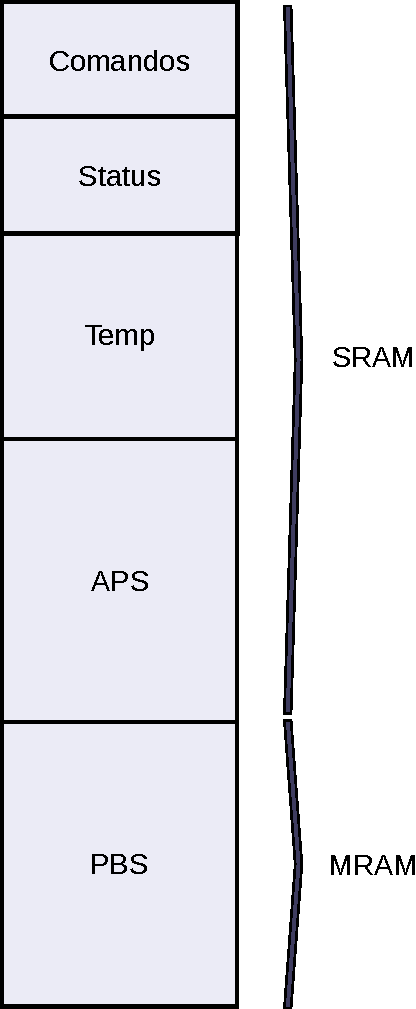
\includegraphics[width=0.3 \columnwidth,]{Figs/memoria.pdf}
	\caption{Alocação de memória proposta}
	\label{fig:mem}
	\end{figure}	 

	%\todo[inline]{}

%	A arquitetura proposta	permite a comunicação do sistema de controle com o experimento utilizando uma rede CAN
%	[11]. As informações coletadas do experimento a serem enviados ao solo (Telemetria - TM) e
%	os comandos recebidos do solo (Telecomandos - TC) são disponibilizadas em uma rede MIL
%	1553[12], um protocolo bastante confiável para a comunicação entre o instrumento e a
%	plataforma. O software proposto é inspirado na experiência do satélite CoRoT com um
%	número reduzido de TC/TM. Sua estrutura é modular, permitindo a utilização de dois a trinta
%	e dois sensores.
	

\section{Bancada de implementação}
	
	A bancada desenvolvida para a implementação do sistema proposto é constituída de um processador Leon 3 com frequência de operação de 60 MHz embarcado em uma FPGA Virtex 5 com dois cores SpaceWire funcionando a 200 Mbps cada, pretende-se com o sistema embarcado simular o experimento. O sistema embarcado possui comunicação com o computador via os dois canais SpW, simulando a interface de comunicação experimento/plataforma, para a ponte SpW-Computador, foi usando um hardware da Star-Dundee desenvolvido para esse fim.  A fim de validar a bancada e possibilitar um estudo do desempenho tanto do protocolo SpW quanto do Leon, uma aplicação que simula o funcionamento de um CCD conectado a uma unidade de processamento.
	
	
\subsection{SpaceWire}

	Um grande esforço tem sido realizado por várias pessoas ligadas à Agência Espacial Européia, à indústria espacial europeia e a área acadêmica no sentido de realizar um aperfeiçoamento e uma padronização das transferências de dados em sistemas embarcados específicos para a área espacial. Um desses esforços tem sido a criação do protocolo Spacewire “ESA ECSS-E-50-12A” de 24 de Janeiro de 2003 e sua atualização em 31 de Julho de 2008 (“ESA ECSS-E-50-12C”).

	Um dos  objetivos da utilização deste protocolo é aumentar a compatibilidade entre subsistemas e componentes aeroespaciais a fim de possibilitar  uma maior reutilização dos mesmos em missões diferentes, como, por exemplo, o reuso de unidades de processamento, unidades de armazenamento de memória, unidades de telemetria, sensores óticos, previamente testados e validados. Esse reuso possibilita além de uma redução de custos como também um menor prazo de desenvolvimento.
	
	O protocolo SpaceWire leva em consideração outros dois padrões, a saber, o IEEE 1355-1995  (IEEE Standard for Heterogeneous InterConnect) e ANSI/TIA/EIA-644 (LVDS). O protocolo SpaceWire provê um link full-duplex, ponto a ponto e serial com taxa máxima de 10Mbps e taxa máxima de 400 Mbps ponto a ponto a uma distancia de no máximo 10 metros.

	Utilizou-se o Codec SpaceWire Light disponível em , \todo{escrever mais}
	
\subsection{Leon 3}

	O LEON3 é um processador de 32-bits baseado na arquitetura SPARC V8, desenvolvido para aplicações embarcadas, combinando alta 	performance com baixa complexidade e baixo consumo energético. Distribuído 	através do VHDL GRLIB IP \cite{GRLIB} sobe licença GPL (\textit{General Public License}) contém além do processador, módulos como: controlador de 	memória, interface PCI, USART, Ethernet MAC. Um exemplo de aplicação das bibliotecas presentes  no GRLIB pode ser visto na Fig \ref{fig:arq}. 

	O processador já é utilizado em diversas missões \cite{},  possui uma versão chamada de Leon3-FT que contém arquitetura enriquecida para detectar e corrigir SEU (\textit{Single Event Upset}) , correção de erros no cache e arquitetura com tripa redundância.

	\begin{figure}[!t]
	\centering
	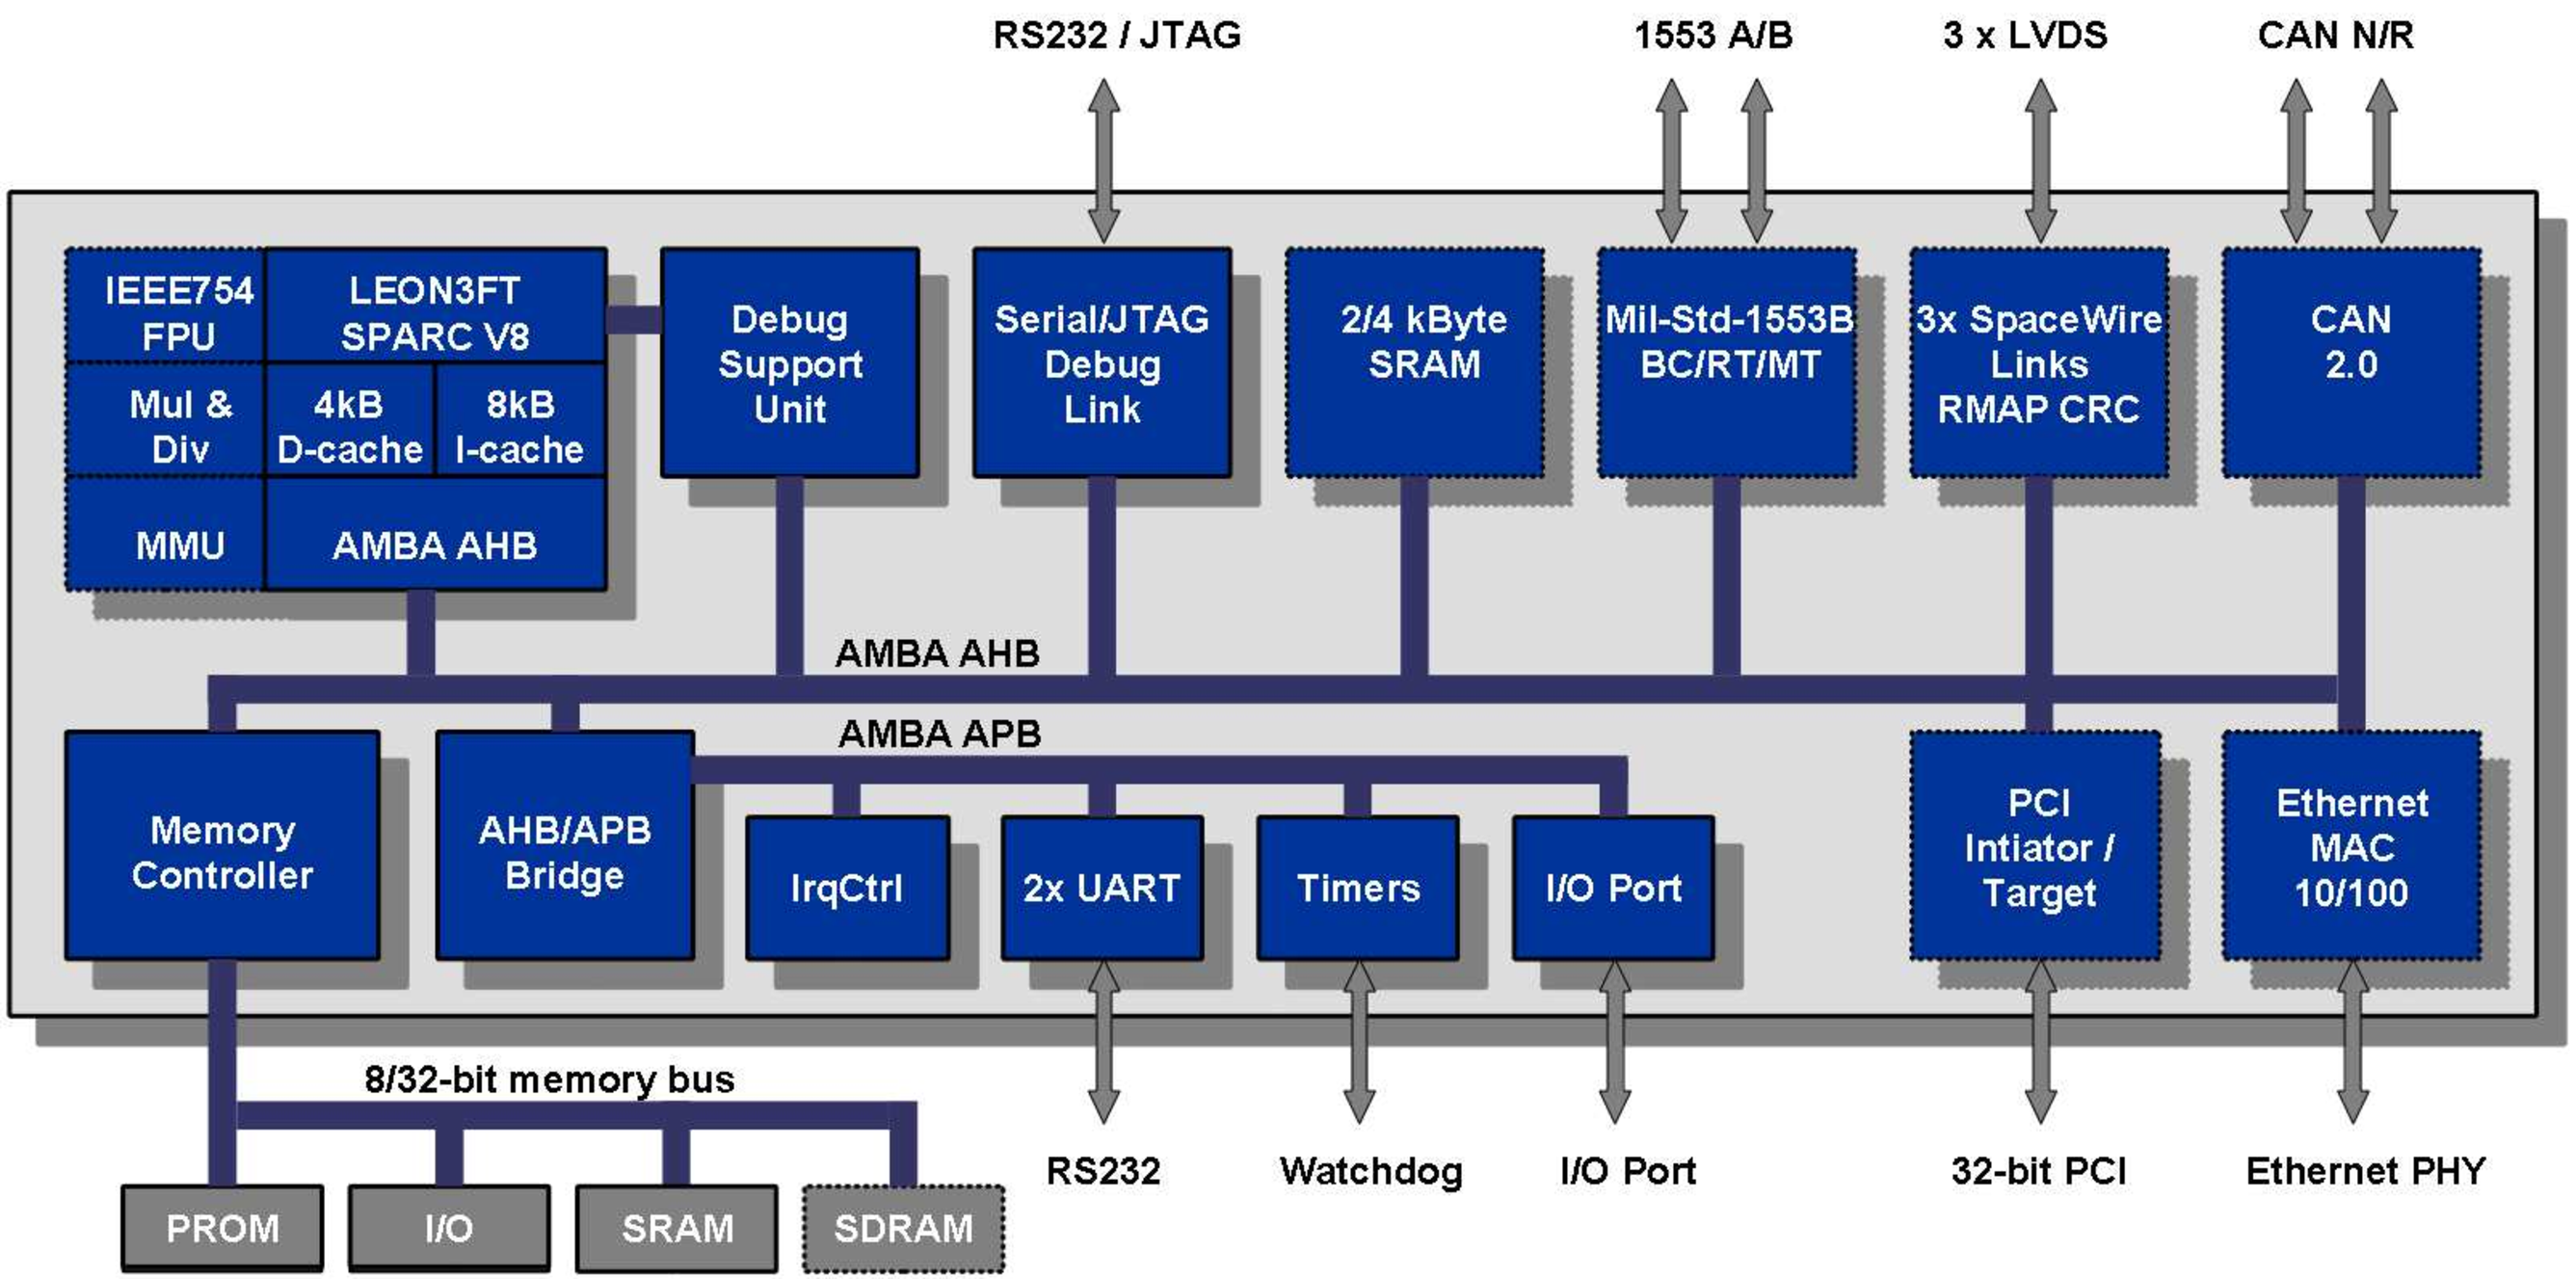
\includegraphics[width=1 \columnwidth,]{Figs/arq.pdf}
	\caption{Biblioteca GRLIB}
	\label{fig:arq}
	\end{figure}	 
	
	O processador LEON3 implementa uma arquitetura Harvard com 	instruções e \textit{cache} de dados separados. Possui divisão e multiplicação	em hardware e uma unidade de processamento de ponto flutuante pode ser 	adicionada. Contém também uma unidade de gerenciamento de memória que	possibilita o mapeamento de 32-bits de endereço virtual e 32-bits de memória. Pode funcionar com múltiplos processadores, os quais podem	compartilham uma mesma memória. 
	
\subsection{Aplicação}

	A aplicação proposta, utiliza a arquitetura da Fig. \ref{fig:bancada} baseada no satélite PLATO \cite{Plato} onde a comunicação do subsistema de imageamento (N-FEE) de utilização científica é feito a partir de dois canais SpW funcionando a 100Mbps casa. O N-FEE é conectado uma unidade de processamento (DPU) responsável pela extração de dados científicos das imagens. Uma nova imagem é transmitida a cada 6s, sendo que a transmissão deve ocupar no máximo 50$\%$ do tempo total.
	
	\begin{figure}[!t]
	\centering
	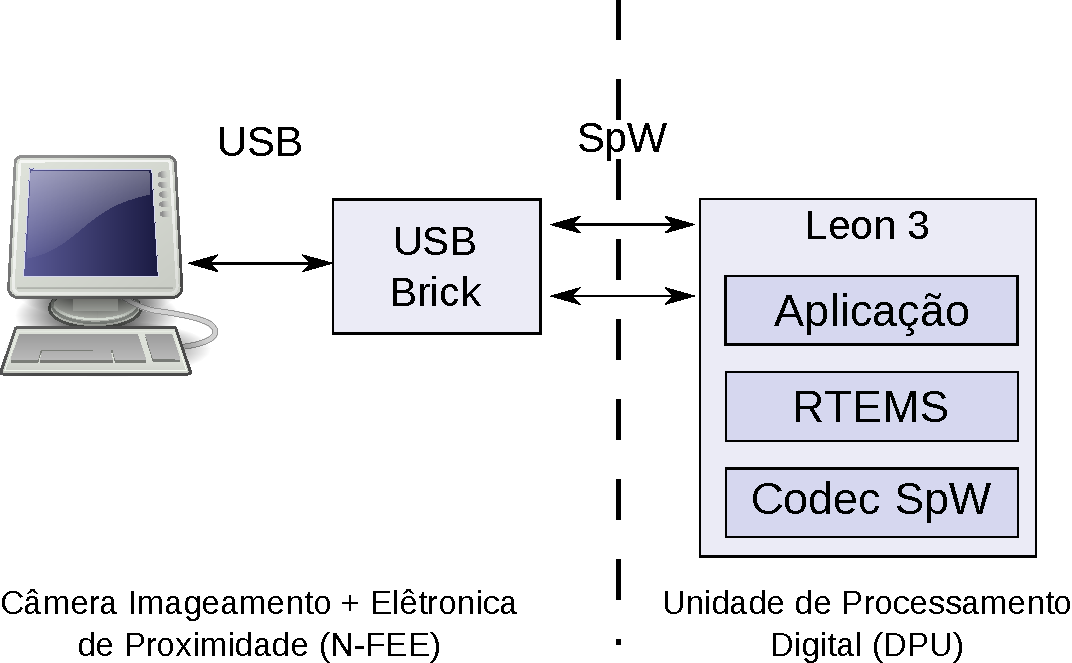
\includegraphics[width=0.8 \columnwidth,]{Figs/bancada.pdf}
	\caption{Bancada desenvolvida para implementação de aplicações aerospaciais}
	\label{fig:bancada}
	\end{figure}	 
	
	A proposta visa emular um sistema real de transmissão de dados entre o N-FEE e a DPU, para tanto desenvolveu-se uma aplicação que utiliza o conjunto computador/ USB-Brick, que possibilita a serialização e envio de imagens ao processador Leon,  podendo assim validar algorítimos de extração de dados voltados para aplicações aerospaciais. Uma futura implementação visa utilizar tal bancada para a implementação da arquitetura  do sistema em tempo real e reconfigurável para controle de experimentos.
	
	Foi utilizado como sistema operacional o RTEMS (\textit{Real-Time Executive for Multiprocessor Systems}) com duas tarefas distintas, uma voltada para recepção de dados (TRX) e outra para transmissão (TTX) da imagem, a comunicação entre tarefas é feito por um \textit{mail box} do TRX ao TTX contendo o endereço da imagem recebida (em memória local), e o tamanho armazenado. Com a proposta conseguiu-se uma taxa de 50Mbps de transmissão, contando latência do link de comunicação e acesso a memória. 
	
\section{Conclusão}	
		
		Nesse trabalho, definiu-se uma topologia robusta capaz de servir como base para o desenvolvimento de softwares para experimentos científicos que necessitem de uma abordagem de tempo real e que possam ser atualizados após lançamento. 
		
		Foi desenvolvido uma bancada para validação e desenvolvimento de aplicações com processador Leon e o protocolo SpaceWire, pretende-se com essa bancada  implementar a proposta de sistema reconfigurável.
	

%\begin{figure}[!t]
%\centering
%\includegraphics[width=2.5in]{myfigure}
% where an .eps filename suffix will be assumed under latex, 
% and a .pdf suffix will be assumed for pdflatex; or what has been declared
% via \DeclareGraphicsExtensions.
%\caption{Simulation Results}
%\label{fig_sim}
%\end{figure}

% Note that IEEE typically puts floats only at the top, even when this
% results in a large percentage of a column being occupied by floats.


% An example of a double column floating figure using two subfigures.
% (The subfig.sty package must be loaded for this to work.)
% The subfigure \label commands are set within each subfloat command, the
% \label for the overall figure must come after \caption.
% \hfil must be used as a separator to get equal spacing.
% The subfigure.sty package works much the same way, except \subfigure is
% used instead of \subfloat.
%
%\begin{figure*}[!t]
%\centerline{\subfloat[Case I]\includegraphics[width=2.5in]{subfigcase1}%
%\label{fig_first_case}}
%\hfil
%\subfloat[Case II]{\includegraphics[width=2.5in]{subfigcase2}%
%\label{fig_second_case}}}
%\caption{Simulation results}
%\label{fig_sim}
%\end{figure*}
%
% Note that often IEEE papers with subfigures do not employ subfigure
% captions (using the optional argument to \subfloat), but instead will
% reference/describe all of them (a), (b), etc., within the main caption.


% An example of a floating table. Note that, for IEEE style tables, the 
% \caption command should come BEFORE the table. Table text will default to
% \footnotesize as IEEE normally uses this smaller font for tables.
% The \label must come after \caption as always.
%
%\begin{table}[!t]
%% increase table row spacing, adjust to taste
%\renewcommand{\arraystretch}{1.3}
% if using array.sty, it might be a good idea to tweak the value of
% \extrarowheight as needed to properly center the text within the cells
%\caption{An Example of a Table}
%\label{table_example}
%\centering
%% Some packages, such as MDW tools, offer better commands for making tables
%% than the plain LaTeX2e tabular which is used here.
%\begin{tabular}{|c||c|}
%\hline
%One & Two\\
%\hline
%Three & Four\\
%\hline
%\end{tabular}
%\end{table}


% Note that IEEE does not put floats in the very first column - or typically
% anywhere on the first page for that matter. Also, in-text middle ("here")
% positioning is not used. Most IEEE journals use top floats exclusively.
% Note that, LaTeX2e, unlike IEEE journals, places footnotes above bottom
% floats. This can be corrected via the \fnbelowfloat command of the
% stfloats package.




% if have a single appendix:
%\appendix[Proof of the Zonklar Equations]
% or
%\appendix  % for no appendix heading
% do not use \section anymore after \appendix, only \section*
% is possibly needed

% use appendices with more than one appendix
% then use \section to start each appendix
% you must declare a \section before using any
% \subsection or using \label (\appendices by itself
% starts a section numbered zero.)
%


\appendices


% use section* for acknowledgement
%\section*{Acknowledgment}


%The authors would like to thank...


% Can use something like this to put references on a page
% by themselves when using endfloat and the captionsoff option.
\ifCLASSOPTIONcaptionsoff
  \newpage
\fi


\bibliographystyle{unsrt}
\addcontentsline{toc}{section}{Referências Bibliográficas}
\bibliography{ref}


% trigger a \newpage just before the given reference
% number - used to balance the columns on the last page
% adjust value as needed - may need to be readjusted if
% the document is modified later
%\IEEEtriggeratref{8}
% The "triggered" command can be changed if desired:
%\IEEEtriggercmd{\enlargethispage{-5in}}

% references section

% can use a bibliography generated by BibTeX as a .bbl file
% BibTeX documentation can be easily obtained at:
% http://www.ctan.org/tex-archive/biblio/bibtex/contrib/doc/
% The IEEEtran BibTeX style support page is at:
% http://www.michaelshell.org/tex/ieeetran/bibtex/
%\bibliographystyle{IEEEtran}
% argument is your BibTeX string definitions and bibliography database(s)
%\bibliography{IEEEabrv,../bib/paper}
%
% <OR> manually copy in the resultant .bbl file
% set second argument of \begin to the number of references
% (used to reserve space for the reference number labels box)
%\begin{thebibliography}{1}

%\bibitem{IEEEhowto:RMAP}
%ESA Requirements and Standards Division, \emph{Space engineering - SpaceWire protocols ECSS-E-ST-50-11C}, Noordwijk, Netherlands, 2008.
%
%\bibitem{IEEEhowto:APPLICATION}
%Alan A., Joseph R., Hennawy, Christopher J., Horace M., \emph{Solar probe plus and spacewire: virtual spacecraft bus}, SpaceWire-2011 Proceedings, The Johns Hopkins University Applied Physics Laboratory, 2011.
%
%\bibitem{IEEEhowto:PLATO}
%Catala, C. and PLATO consortium, \emph{PLATO PLAnetary Transits and Oscillations of stars – A study of exoplanetary systems, proposal}, Vol. 1, Available in: Lesia, \emph{$http://www.lesia.obspm.fr/perso/claude-catala/plato_web.html$}, Accessed 20 Feb. 2011.
%
%\bibitem{IEEEhowto:SpW}
%ESA Requirements and Standards Division,   \emph{SpaceWire links, nodes, routers and networks ECSS-E-ST-50-11C}, Noordwijk, Netherlands, 2008.
%
%\bibitem{IEEEhowto:Leon2}
%Gaisler research,   \emph{LEON2 Processor User’s Manual}, Version 1.0.30, 2005.
%
%\bibitem{IEEEhowto:StarDundee}
%Star Dundee, \emph{SpaceWire Brick Hardware Users Manual - UoD BRICK USER}, Version 1.0, 2004.
%
%\bibitem{IEEEhowto:AMBA}
%ARM, \emph{AMBA Specification ARM IHI 0011A}, Inssue A, first release, 1999.




%\end{thebibliography}




% that's all folks
\end{document}


